\documentclass[a4paper,11pt]{article}

\usepackage{cmap}		
%\usepackage[utf8]{inputenc}			
\usepackage[spanish]{babel}
\usepackage{framed}
\usepackage{hyperref}
\usepackage{amsmath}
\usepackage{graphicx}
\usepackage[colorinlistoftodos]{todonotes}
\usepackage{wrapfig}
\usepackage{lipsum}
\usepackage{listings}
\usepackage{color}
\usepackage{indentfirst}
\usepackage{times}
\usepackage{textcomp}
\usepackage{pgfgantt}
\usepackage{lipsum}
\usepackage{csquotes}

% set document font, font sizes, margin dimensions and spacing
\usepackage{fontspec}
\setmainfont{Arial}
\usepackage[top=15mm,bottom=25mm,left=20mm,right=20mm]{geometry}
\usepackage{setspace}\onehalfspacing
\usepackage{titlesec}
\titleformat*{\section}{\Large\bfseries}
\titleformat*{\subsection}{\Large\bfseries}
\titleformat*{\subsubsection}{\Large\bfseries}
\titleformat*{\paragraph}{\Large\bfseries}
\titleformat*{\subparagraph}{\Large\bfseries}
\setlength{\parskip}{0.6em}

\newif\ifblackandwhite
\blackandwhitetrue

\usepackage{etoolbox}
\usepackage{longtable}%
\AtBeginEnvironment{longtable}{%
  \addfontfeature{RawFeature=+tnum;-onum}%  <--- requires LuaTeX
}

\usepackage{pdflscape}
%\usepackage[svgnames]{xcolor}
 \usepackage{colortbl}%
   \newcommand{\myrowcolour}{\rowcolor[gray]{0.925}}
\usepackage{booktabs}

\ifblackandwhite
  \newcommand{\cheading}[2]{\textbf{#1\hfill #2}}
  \newcommand{\highest}[1]{\textbf{#1}}% == highest score for question
\else
  \newcommand{\cheading}[2]{\textcolor{Maroon}{\textbf{#1\hfill #2}}}
  \newcommand{\highest}[1]{\textcolor{Maroon}{\textbf{#1}}}%
\fi

\definecolor{mygray}{rgb}{0.4,0.4,0.4}
\definecolor{mygreen}{rgb}{0,0.8,0.6}
\definecolor{myorange}{rgb}{1.0,0.4,0}

\lstdefinestyle{customc}{
  belowcaptionskip=1\baselineskip,
  breaklines=true,
  frame=L,
  xleftmargin=\parindent,
  language=C,
  showstringspaces=false,
  basicstyle=\footnotesize\ttfamily,
  keywordstyle=\bfseries\color{green!40!black},
  commentstyle=\itshape\color{purple!40!black},
  identifierstyle=\color{blue},
  stringstyle=\color{orange},
  numbers=left,
  numbersep=12pt,
  numberstyle=\small\color{mygray},
}
\lstset{escapechar=@,style=customc}

\newcommand{\HRule}{\rule{\linewidth}{0.5mm}}

%Definindo um comando todoin que aceita quebra de linha e fórmulas
\newcommand\todoin[2][]{\todo[inline, caption={2do}, #1]{
\begin{minipage}{\textwidth-4pt}#2\end{minipage}}}

\newcommand\todogeg[2][]{\todo[inline, caption={#2}, color=yellow!100, #1]{
\begin{minipage}{\textwidth-4pt}#2\end{minipage}}}

\newcommand\todovwcm[2][]{\todo[inline, caption={#2}, color=red!100, #1]{
\begin{minipage}{\textwidth-4pt}#2\end{minipage}}}
\begin{document}
\begin{titlepage}
\begin{center}

% logo

\includegraphics[width=0.5\textwidth]{images/logo-udea.png}~
\\[2cm]



% identificação do relatório
\HRule \\[0.4cm]
{\large \bfseries PROYECTO DE INVESTIGACIÓN: INTERRUPCIONES \\
[0.4cm]}
\HRule 
\\[2cm]

% identificação do aluno
\large\textbf{ALUMNO}\\[1cm]
ANDREA OSPINA HINCAPIÉ\\
andrea.ospinah@udea.edu.co\\
INFORMÁTICA II \\
 INGENIERÍA ELECTRÓNICA
\\[1.5cm]

% identificação do orientador
\large\textbf{DOCENTE}\\[1cm]
AUGUSTO ENRIQUE SALAZAR JIMÉNEZ\\
DEPARTAMENTO DE INGENIERÍA ELECTRÓNICA Y TELECOMUNICACIONES
\\[1cm]



\vfill

% Bottom of the page
{\large \textbf{3 DE JULIO DE 2020}}

\end{center}
\end{titlepage}

\newpage
\centerline{{\large\bfseries PROYECTO DE INVESTIGACIÓN: INTERRUPCIONES}}
El concepto de las interrupciones es un concepto de suma relevancia para comprender por completo el funcionamiento de los microprocesadores. Si bien existen diferencias en la forma como estas pueden ser implementadas según el microprocesador que se esté utilizando, existen aspectos generales de las interrupciones que se presentarán a continuación por medio de la respuesta a importantes preguntas: 

{\large\bfseries ¿Qué es una interrupción en el contexto de los microprocesadores?} 

Una interrupción, como podría dar a entender su nombre, es una señal \cite[p.217]{burrell2003fundamentals} que es enviada al microcontrolador para que, por medio de un mecanismo de interrupciones \cite[p.217]{burrell2003fundamentals} se detenga el programa principal, de manera que se genere una respuesta, conocida como ISR (\emph{Interrupt Service Routine}), y posteriormente se continúe el programa principal en el punto en el que fue interrumpido \cite[p.1]{reyes2015arduino}.
Para comprender por completo este concepto puede pensarse en una gran empresa con múltiples departamentos como el departamento de marketing, el departamento financiero, o el departamento de desarrollo, además de tener un presidente que se encuentra realizando una tarea (programa principal). De repente el presidente recibe una llamada del jefe del departamento de marketing (interrupción) en la cual le indica que es necesario hacer una reunión para discutir la publicidad de un nuevo producto. El presidente procede entonces a convocar una reunión (subrutina). Al finalizar esta reunión el presidente continúa con sus tareas hasta que reciba una nueva llamada del mismo u otro departamento. La situación anterior es, entonces, un ejemplo de cómo funciona el concepto de las interrupciones.



{\large\bfseries ¿Se puede hablar de la historia de las interrupciones?} 

Existe un claro antecedente del concepto de interrupción: el \emph{polling}, el cual consiste en que el microprocesador realice un monitoreo constante de un evento \cite[p.1]{reyes2015arduino}. 

Continuando con el ejemplo de la empresa, el \emph{polling} sería equivalente a que en lugar de que el presidente reciba la llamada de los departamentos, este se encargue de llamarlos constantemente hasta que la tarea asignada a cada departamento sea completada y se pueda realizar la reunión. Este mecanismo fue reemplazado en los microcontroladores por una unidad de interrupciones ya que el \emph{polling} es poco eficiente y tiene el potencial de causar la pérdida de información importante sobre los eventos o sobre el programa principal \cite[p.2]{reyes2015arduino}.

En términos de implementación se le atribuye el primer uso de interrupciones a distintas máquinas, por ejemplo, la UNIVAC 1103 (1953) suele ser mencionada como una de las primeras computadoras en utilizar un sistema de interrupciones \cite[p.181]{historia1}por algunos autores. Sin embargo en su manual original estas no son mencionadas \cite{smotherman_2017}. Por tanto también suele atribuirse el primer uso de interrupciones a la UNIVAC 1103A (1956)\cite{smotherman_2017}\cite{historia2}.

{\large\bfseries ¿Que tipo de interrupciones existen? }

Existen múltiples tipos de interrupciones pero se destacan los siguientes:

{\large\bfseries -Interrupciones de hardware vs interrupciones de software:}
Las interrupciones de software son aquellas que se producen internamente por una instrucción llamada explícitamente dentro del conjunto de instrucciones que se ejecutan por el microprocesador. Por otro lado, las interrupciones de hardware pueden subdividirse a su vez en interrupciones de hardware internas e interrupciones de hardware externas. Las interrupciones de hardware externas son aquellas producidas por periféricos o hardware diferente al procesador principal, mientras que las interrupciones de hardware internas son las generadas por limitaciones del hardware para ejecutar instrucciones como operaciones matemáticas ilegales \cite{labrosse2008embedded}.

{\large\bfseries -Vectorizadas vs no vectorizadas: }
Como se explicará en las siguientes preguntas, las ISR suelen ser almacenadas en un vector en la memoria del microcontrolador. Las interrupciones vectorizadas son aquellas cuyas ISR tienen una posición predefinida en el vector, mientras que para las no vectorizadas, al ser estas recibidas por el microcontrolador, este envía una señal para que el hardware externo envíe el vector de interrupción donde se encuentra la ISR. \cite[p.195]{udayashankara2009microcontroller}

{\large \bfseries -Enmascarables vs no enmascarables: }
Las interrupciones enmascarables son aquellas que pueden ser ocultadas al procesador cuando no es deseable que se interrumpa el programa principal. Este control puede realizarse por medio de software de manera global(activando o desactivando todas las interrupciones) o de manera individual. Las interrupciones no enmascarables son aquellas que, sin importar el estado global de las interrupciones, es necesario que sean transmitidas al procesador. Este último es el caso de interrupciones como RESET \cite[p.11]{susnea2005microcontrollers}.

{\large\bfseries ¿Cómo se hace la implementación de interrupciones a nivel de hardware? } 

A nivel de hardware, y para realizar el control de interrupciones, se utiliza un dispositivo denominado unidad de interrupciones, el cual se encarga de indicarle al microprocesador cuándo se presenta una interrupción de manera que pueda ser atendida.
De esta forma el microprocesador consultará los vectores de interrupciones donde se encuentran almacenadas, en orden de prioridad, la dirección en memoria de las ISR que corresponden a cada interrupción o una instrucción para que se ejecute la ISR \cite[p.9]{susnea2005microcontrollers}. Adicionalmente, al producirse una interrupción, debe guardarse (normalmente en el stack) la información del estado del procesador (registros y banderas) antes de atender la interrupción para que sea posible retornar al programa principal una vez la ISR sea ejecutada \cite[p.4]{reyes2015arduino}. Este último aspecto puede variar dependiendo del microcontrolador utilizado así que es responsabilidad del programador asegurarse de que se guarde la información necesaria del procesador \cite[p.10]{susnea2005microcontrollers}.
Por último, para el caso en el que presenten varias interrupciones de manera simultánea, éstas suelen ser ejecutadas en orden de prioridad según una lista que se haya definido, por medio del hardware,en cada microcontrolador. Esta lista no puede ser cambiada.

{\large\bfseries ¿Cómo se implementan las interrupciones por software?  } 

Para la el manejo de interrupciones el software puede jugar distintos papeles como brindar el control de  enmascarar o no interrupciones que se presenten por hardware.
En el caso de interrupciones de software existen microcontroladores que las implementan como forma de comunicación con el sistema operativo. Este tipo de interrupciones también son conocidas como llamadas al sistema y en los microcontroladores en que son implementadas suelen permitir que se cambie entre modo supervisor y modo usuario \cite[p.236]{rafiquzzaman1995microprocessors}.
Para que se pueda realizar este último proceso es necesario tener una interfaz llamada la \emph{Application Binary Interface }(ABI), en la cual se tienen definidos aspectos como las llamadas al sistema y las instrucciones asociadas a estas. la ABI, como su nombre lo indica, utiliza lenguaje máquina por lo que es independiente de cualquier lenguaje de programación. Sin embargo, los aspectos definidos en esta, y que son utilizados para interrupciones de software, dependen de la arquitectura del microcontrolador \cite[p.24]{ecker2009hardware}.

{\large\bfseries Implementación de interrupciones} 

Para la implementación de interrupciones con arduino debe considerarse:

{\large\bfseries Interrupciones en Arduino Uno} 

Para Arduino Uno existen interrupciones externas asociadas a las interrupciones IN0 e IN1 que se encuentran en los pines digitales 2 y 3. Para la activación de las interrupciones solo se permiten los modos LOW (pin en 0V), CHANGE (se presenta cambio de estado), RISING (cambio de bajo a alto) y FALLING (cambio de alto a bajo). Además, para declarar variables que se modificarán en la ISR se declaran como volatile y es importante que la ISR creada no contenga delays y sea lo más simple posible. \cite[p.11-14]{reyes2015arduino}.
Para especificar las subrutinas se utiliza la siguiente función:
\begin{verbatim}attachInterrumpt(PinToAttach,ISR_Name,Mode);\end{verbatim}
Con una ISR de tipo void y que no reciba parámetros.

{\large\bfseries Ejemplo de implementación} 

El siguiente ejemplo utiliza dos pulsadores para generar interrupciones a un programa principal en el que se encienden y apagan dos LEDs durante un periodo definido por una variable, la cual será modificada por medio de una interrupción creada al presionar uno de los pulsadores, de manera que el periodo disminuya de manera que no sea menor a un periodo mínimo definido en el programa.
Adicionalmente, el segundo pulsador creará una interrupción cuyo efecto será apagar los LEDs oscilantes y encender un tercer LED durante tres segundos. Esto se presentará una vez se haya finalizado la oscilación de los LEDs que se está ejecutando en el momento en que se presiona el pulsador.

En la siguiente imagen se presentan las conexiones realizadas para la implementación del ejemplo:

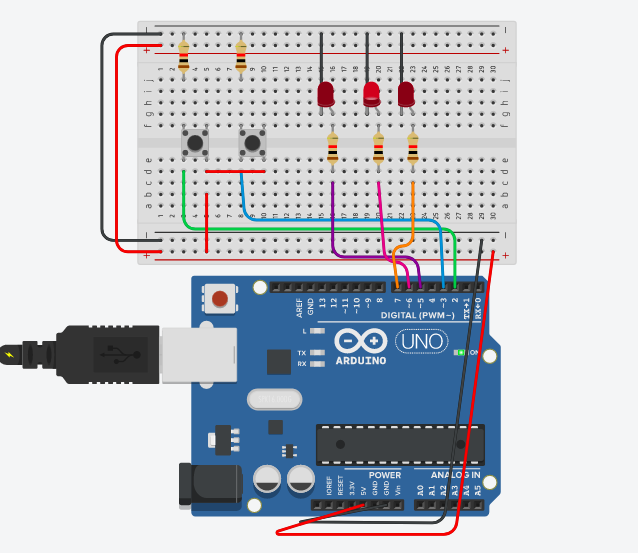
\includegraphics[width=0.4\textwidth]{images/Conexiones.png}~

{\large\bfseries Imagen: Conexiones de ejemplo de implementación}

El código fuente (EjemploInterrupciones.ino) de la implementación puede encontrarse en \href{https://github.com/AndreaOspinaHincapie/Informatica2/tree/master/Proyectos%20de%20investigaci%C3%B3n/Interrupciones}{\underline {este}} repositorio.

Y un video del funcionamiento del ejemplo se encuentra en este link:  \url{https://www.youtube.com/watch?v=WgSvHcRHfT4&feature=youtu.be}


\newpage

\renewcommand\refname{REFERENCIAS BIBLIOGRÁFICAS}
%\bibliographystyle{abntex2-alf}
\bibliographystyle{IEEEtran}
\bibliography{referencias.bib}
%\listoftodos

\end{document}